% !TeX program = xelatex
% !TeX encoding = UTF-8
\documentclass[UTF8,a4paper,zihao=-4,fontset=fandol]{ctexart}
% !TeX root = main.tex
% 中文字体随 TeX Live 提供，可随工程迁移，不依赖 Windows 专用字体。
\usepackage[left=25mm,right=25mm,top=25mm,bottom=25mm]{geometry}
\setmainfont{texgyretermes-regular.otf}[
  BoldFont=texgyretermes-bold.otf,
  ItalicFont=texgyretermes-italic.otf,
  BoldItalicFont=texgyretermes-bolditalic.otf]
\usepackage{amsmath,amssymb}
\usepackage{graphicx}
\usepackage{placeins}
\usepackage[font=small,labelfont=bf,labelsep=quad,
            justification=justified,singlelinecheck=false]{caption}
\usepackage{booktabs}
\usepackage{enumitem}
\usepackage[superscript,nomove]{cite}
% 保留原稿的方括号上标引文格式。
\makeatletter
\renewcommand{\@citess}[1]{\textsuperscript{\normalfont[#1]}}
\makeatother
\usepackage[unicode,hidelinks]{hyperref}
\hypersetup{pdftitle={CMSRN 中文论文}}
\ctexset{
  section={format=\Large\bfseries,number=\arabic{section},
           beforeskip=1.2ex plus 0.5ex,afterskip=0.8ex plus 0.2ex},
  subsection={format=\large\bfseries,beforeskip=1ex plus 0.3ex,
              afterskip=0.6ex plus 0.2ex}
}
\linespread{1.2}
\setlength{\parindent}{2em}
\setlength{\parskip}{0pt}
\setlength{\emergencystretch}{2em}
\setlist[enumerate]{leftmargin=2em,label=\arabic*.,itemsep=0.25em,topsep=0.4em}
\providecommand{\tightlist}{\setlength{\itemsep}{0pt}\setlength{\parskip}{0pt}}
\allowdisplaybreaks[1]
\clubpenalty=10000
\widowpenalty=10000
\raggedbottom
\pagestyle{plain}

% Compact, readable float placement; retain the original font size and margins.
\DeclareCaptionFont{compact}{\linespread{1.05}\selectfont}
\captionsetup{font={small,compact},skip=5pt}
\setlength{\textfloatsep}{11pt plus 2pt minus 2pt}
\setlength{\floatsep}{9pt plus 2pt minus 2pt}
\setlength{\intextsep}{10pt plus 2pt minus 2pt}
\renewcommand{\topfraction}{0.95}
\renewcommand{\bottomfraction}{0.90}
\renewcommand{\textfraction}{0.05}
\renewcommand{\floatpagefraction}{0.75}
\setcounter{topnumber}{4}
\setcounter{bottomnumber}{3}
\setcounter{totalnumber}{6}
\makeatletter
\setlength{\@fptop}{0pt}
\setlength{\@fpsep}{10pt}
\setlength{\@fpbot}{0pt plus 1fil}
\makeatother
\AtBeginDocument{%
  \setlength{\abovedisplayskip}{8pt plus 2pt minus 2pt}%
  \setlength{\belowdisplayskip}{8pt plus 2pt minus 2pt}%
  \setlength{\abovedisplayshortskip}{3pt plus 1pt minus 1pt}%
  \setlength{\belowdisplayshortskip}{6pt plus 1pt minus 1pt}}

% Keep each figure/table inside its owning section, subsection and subsubsection.
\AddToHook{cmd/section/before}{\FloatBarrier}
\AddToHook{cmd/subsection/before}{\FloatBarrier}
\AddToHook{cmd/subsubsection/before}{\FloatBarrier}

\hypersetup{pdftitle={CMSRN 实验分析补充材料}}
\ctexset{section/number={S\arabic{section}}}
\renewcommand{\thefigure}{S\arabic{figure}}
\renewcommand{\thetable}{S\arabic{table}}
\renewcommand{\theequation}{S\arabic{equation}}
\begin{document}
\begin{center}\Large\bfseries CMSRN：实验分析补充材料\end{center}

\section{分组与固定输出诊断}

分析以成都1,723个、上海1,781个真实测试窗口为基础，每个窗口覆盖1,024个网格；各城市使用一套联合预测流入和流出的模型权重，两个通道分别统计。H6为提前30分钟预测单个5分钟流量桶，H1--H12为5--60分钟。预测保持原始连续输出，不截断、取整或平滑。

常规参考使用固定训练窗口覆盖的去重历史时间点拟合，仅保留来源质量正常的时刻。对每个网格和通道，按工作日/周末类型及五分钟时间槽取流量中位数；某类型--时间槽不足4个观测时，合并两种日期类型在同一时间槽的观测，若该时间槽仍无观测，则回退至该网格、通道的训练流量中位数。日历使用实际北京时间。

令\(v_{\tau,i,c}=x_{\tau,i,c}-m_{\tau,i,c}\)为扣除常规参考后的流量，\(\mathcal F\)为上述有效训练时间点集合。对每个网格\(i\)和通道\(c\)单独计算固定尺度
\begin{equation}
 s_{i,c}=\max\!\left\{1,\;1.4826\,\operatorname{median}_{\tau\in\mathcal F}
 \left|v_{\tau,i,c}-\operatorname{median}_{u\in\mathcal F}v_{u,i,c}\right|\right\}.
\end{equation}
外部分析的标准化残差为\(r_{\tau,i,c}=v_{\tau,i,c}/s_{i,c}\)。1计数的下限避免稀疏流量位置因尺度过小而被过度放大。尺度按网格和通道固定，不随预测步或测试窗口重估。

阈值拟合仅使用12个历史时刻均来源可用的训练窗口，覆盖全部网格并按城市、通道分别统计。成都常规参考使用5,181个去重时间点、阈值使用5,170个窗口；上海分别为4,202个时间点和4,180个窗口。来源质量筛选只服务于此次外部分析，未改变已有预测实验的训练时间轴及标准化统计。

对每个预测起点、网格和通道定义
\begin{equation}
  D=\frac{1}{12}\sum_{k=1}^{12}|r_k|,
  \qquad U=\frac{1}{11}\sum_{k=2}^{12}|r_k-r_{k-1}|.
\end{equation}
\(D\)描述相对常规参考的历史偏离，\(U\)描述近期变化强度。设\(\mathcal{C}_i\)为目标网格\(i\)的有效固定候选源集合，\(\bar r_i\)为该网格历史12步标准化残差均值，则候选背景差异为
\begin{equation}
  B_i=\frac{1}{|\mathcal{C}_i|}\sum_{j\in\mathcal{C}_i}|\bar r_i-\bar r_j|.
\end{equation}
候选集合及其有效掩码沿用模型的固定支持。\(B_i\)为历史流量构造的外部代理，与BCMS内部学习到的低频表征分别定义。

\begin{table}[!htbp]
\centering\small
\caption{训练期拟合并冻结的分组规则}
\begin{tabular}{p{0.16\linewidth}p{0.29\linewidth}p{0.45\linewidth}}
\toprule
分组量 & 阈值拟合范围 & 测试分组 \\
\midrule
偏离分数\(D\) & 训练历史 & Q50、Q80、Q95划分Low、Moderate、High、Extreme；等于边界归较低组。\\
近期变化\(U\) & 训练\(D>\mathrm{Q80}\) & 超过Q75为Rapid，其余为Slow。\\
背景差异\(B\) & 训练\(D>\mathrm{Q80}\) & 第\(1/3\)、\(2/3\)分位数划分Low、Medium、High。\\
\bottomrule
\end{tabular}
\end{table}


\begin{table}[!htbp]
\centering\footnotesize
\caption{两城市的训练分组阈值（显示至六位小数）}
\setlength{\tabcolsep}{4pt}
\begin{tabular}{llrrrrrr}
\toprule
城市 & 通道 & \(D_{50}\) & \(D_{80}\) & \(D_{95}\) & \(U_{75}\) & \(B_{1/3}\) & \(B_{2/3}\) \\
\midrule
成都 & 流入 & 0.166667 & 0.583333 & 1.083333 & 1.636364 & 0.279326 & 0.453125 \\
成都 & 流出 & 0.166667 & 0.625000 & 1.083333 & 1.636364 & 0.287192 & 0.471179 \\
上海 & 流入 & 0.281038 & 0.708333 & 1.096048 & 1.636364 & 0.311065 & 0.489387 \\
上海 & 流出 & 0.250000 & 0.674491 & 1.083333 & 1.590909 & 0.311294 & 0.492517 \\
\bottomrule
\end{tabular}
\par\smallskip\footnotesize 实际分组使用未舍入阈值；\(U\)和\(B\)的分位数均在训练\(D>D_{80}\)的子集中拟合。
\end{table}

所有阈值按城市和通道分别拟合。高偏离子集为High与Extreme的并集，即\(D>\mathrm{Q80}\)；背景差异的High组与偏离程度的High组属于不同划分。测试组别仅由已观测历史决定，跨预测步保持固定。各步使用\(y>0\)掩码计算组内MAE，因此有效样本--网格数随预测步变化；训练分位数也不意味着测试组别具有相同比例。图中\(n\)为有效评估位置数，不是独立训练次数。

固定输出诊断扣除实际加入预测的残差，包含原门控权重、可学习强度与逆标准化尺度；模型参数、其他输出和门控保持不变。SERR自身项扣除的是已加权的自身预测与基础预测之差，时滞项扣除的是已加权时滞修正；BCMS扣除完整的跨区域修正。各残差的移除MAE差值衡量其对组平均误差的净作用，由于绝对值损失的非线性，不同项的差值不能直接相加。该诊断使用主要对比实验的模型，与正文5.3节基于另一轮Full对照的独立重训练消融分别报告。

\FloatBarrier
\section{全部方法的绝对误差}

补充图~\ref{fig:supp-scenario-absolute}给出H6分组MAE，包含CMSRN与16种基线，补充正文的相对改善率。CMSRN在Extreme组的误差仍明显高于Low组，且较高偏离组伴随更大的流量规模。例如，成都流入的正目标均值由Low组的1.160增至Extreme组的3.637，上海流出由1.157增至4.068。绝对误差与相对排名反映不同侧面；相近流量规模下的交叉分层可进一步检验偏离程度与误差之间的关系。

\begin{figure}[!htbp]
\centering
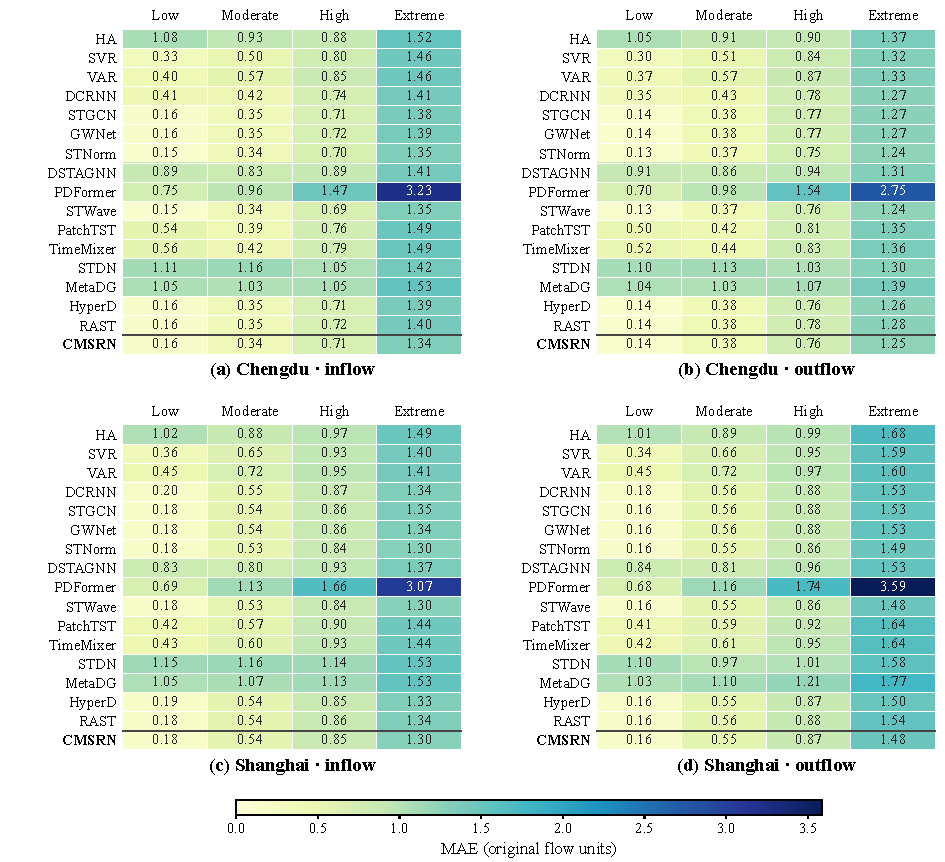
\includegraphics[width=\linewidth]{figures/scenarios/performance_h6_absolute_mae_paper.pdf}
\caption{全部17种方法在四个历史偏离组上的H6绝对MAE，单位为原始5分钟流量计数。四面板使用统一色标，颜色越深表示误差越大。图内保留两位小数，显示相同不等于精确指标并列；分组和正目标掩码与正文相对性能图一致。}
\label{fig:supp-scenario-absolute}
\end{figure}
\FloatBarrier

\section{完整测试集上的BCMS残差作用}

补充图~\ref{fig:supp-scenario-bcms-all}将样本范围扩展至完整测试集，沿用训练高偏离历史拟合的背景分组阈值。全部144个背景组--预测步单元的移除差值均为正，各对应单元的数值均高于仅高偏离子集的结果，并保持低背景差异组高于中等组、中等组高于高差异组的顺序。以上海流入H6为例，完整测试集三个背景组的差值依次为0.023927、0.014393和0.008673，高偏离子集则为0.012448、0.008885和0.006301。两种分析范围具有包含关系；本图说明BCMS的平均修正收益覆盖更广的交通状态。

\begin{figure}[!htbp]
\centering
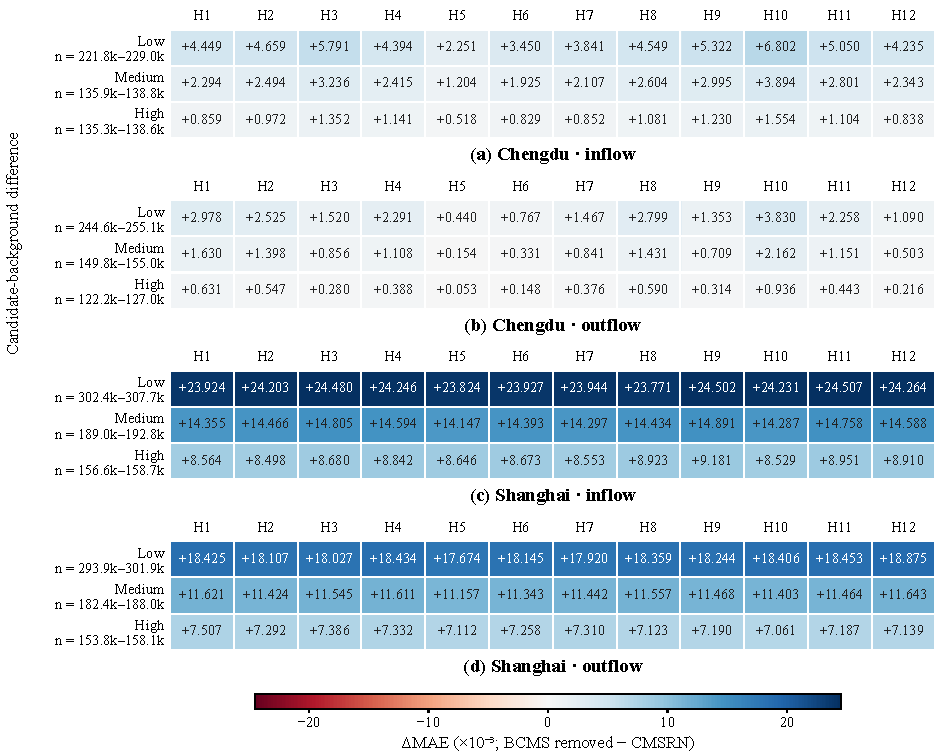
\includegraphics[width=\linewidth]{figures/scenarios/bcms_sensitivity_horizons_all_test_paper.pdf}
\caption{完整测试集上的BCMS固定输出移除敏感性。每格为\(1000\times\Delta\mathrm{MAE}\)，正值表示原残差降低组平均MAE；H1--H12对应5--60分钟。\(n\)为跨步的有效样本--网格数范围。组别与正文高偏离分析采用相同阈值。本图四面板色标统一，但范围不同于高偏离专图，跨图比较应读取数值。}
\label{fig:supp-scenario-bcms-all}
\end{figure}
\FloatBarrier

\section{消融实验的分通道结果}\label{sec:supp-ablation}

表~\ref{tab:supp-ablation-channels}列出成都T5数据集上完整CMSRN与三个独立重训练变体的分通道及联合结果。测试排除批次补齐样本，仅统计\(\mathrm{target}>0\)的位置，先分别计算每个预测步的指标，再对12步取平均。联合MAE和联合RMSE均为流入、流出相应AVG12指标的等权平均，其中联合RMSE按通道指标平均计算。

% !TeX root = ../supplementary-scenarios.tex
\begin{table}[!htbp]
  \centering
  \caption{成都T5消融实验的分通道与联合AVG12指标}
  \label{tab:supp-ablation-channels}
  \begingroup
  \linespread{1}\fontsize{9}{11}\selectfont
  \setlength{\tabcolsep}{3pt}
  \renewcommand{\arraystretch}{1.08}
  \begin{tabular*}{\linewidth}{@{\extracolsep{\fill}}lrrrrrr@{}}
    \toprule
    模型配置 & 流入MAE & 流入RMSE & 流出MAE & 流出RMSE & 联合MAE & 联合RMSE \\
    \midrule
    CMSRN & \textbf{0.708421} & \textbf{1.293545} & 0.708654 & 1.223468 & \textbf{0.708537} & \textbf{1.258507} \\
    w/o Self Expert (A1) & 0.711386 & 1.301713 & 0.711155 & \textbf{1.222889} & 0.711270 & 1.262301 \\
    w/o Delay Expert (A2) & 0.709032 & 1.302225 & 0.708673 & 1.223911 & 0.708852 & 1.263068 \\
    w/o BCMS (A3) & 0.708573 & 1.295331 & \textbf{0.708567} & 1.223305 & 0.708570 & 1.259318 \\
    \bottomrule
  \end{tabular*}
  \par\vspace{3pt}
  \begin{minipage}{\linewidth}\footnotesize
  注：加粗表示列内最低误差；联合指标按两通道等权平均，所列值保留六位小数。
  \end{minipage}
  \endgroup
\end{table}

\FloatBarrier

\end{document}
